\section{Evaluation}
\label{sec:evaluation}

Extensions implemented in ServiceMix-mt may affect on its performance, and system's resources consumption. Therefore, in this section we focus on evaluating, in the first place, the operative system's resources the \ac{ESB} consumes. In the second place, we evaluate the difference between connecting directly to the backend Cloud or local data store (without transparency to the user), and the utilization of a transparent connection through the Cloud-Enabled Data Access Bus. For evaluation purposes we utilize the TPC-H benchmark for generating the data, and Apache JMeter for performing the load tests. 

\subsection{TPC-H Benchmark}

The TPC-H benchmark is a set of libraries written in the C language which provide support for generating large volumes of data for populating the database system which wants to be evaluated \cite{tcpbenchmark}. Furthermore, it generates queries with a high degree of complexity to be executed on the databases where the generated data is stored. In this diploma thesis we utilize the TPC-H benchmark to generate the data which is stored in the local MySQL database system, and in the backend MySQL database instances hosted in Amazon RDS. The data generated by the benchmark varies in size, and is stored in a database which follow the schema described in Figure \ref{fig:tpchschema}. 

\begin{figure}[htb]
	\centering
		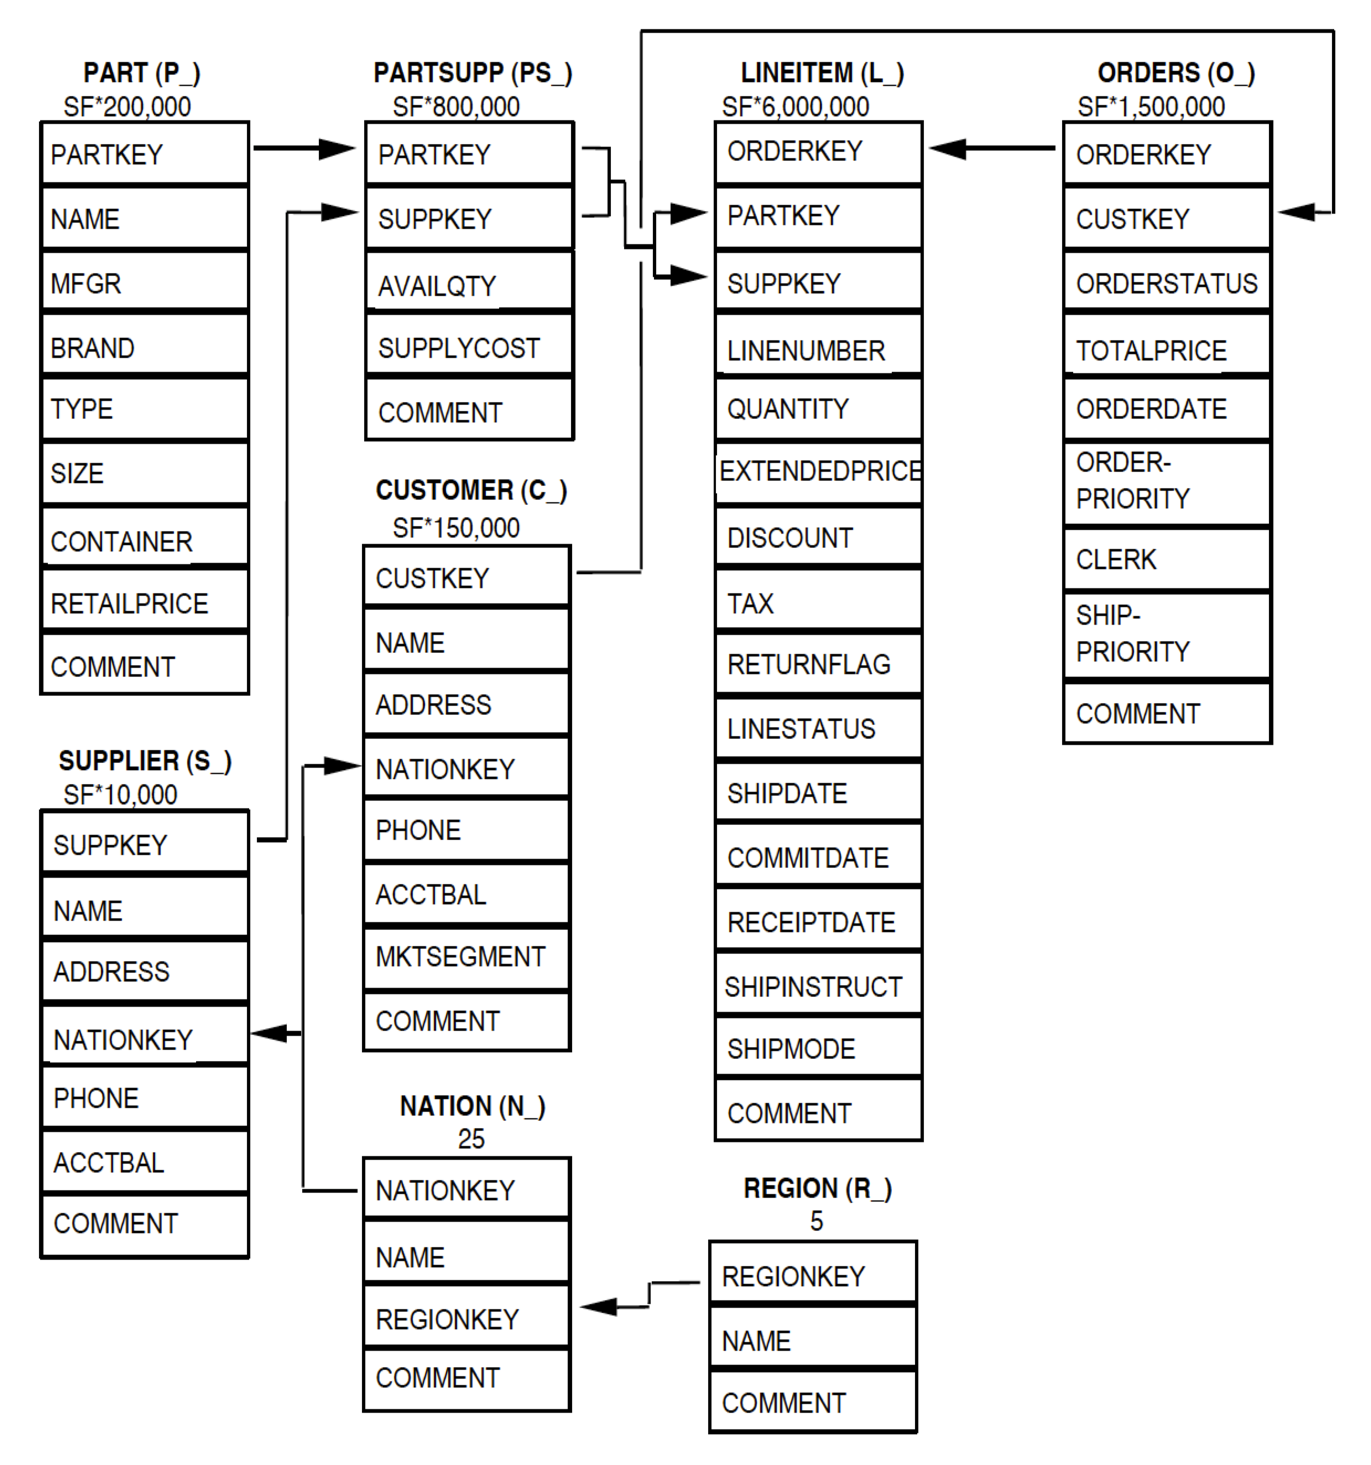
\includegraphics[clip, scale=0.5]{./gfx/tpchdbschema.pdf}
	\caption[TPC-H Database Schema]{TPC-H database schema generated \cite{tcpbenchmark}.}
	\label{fig:tpchschema}
\end{figure}

The TPC-H data and queries generator operations are mainly managed in two executables, which are generated by building the library with the \term{make} command: \term{dbgen}, and \term{qgen}. The former has as input option the size, which we set in this diploma thesis to 1GB, while the latter generates a set of queries for the generated data. After the data and queries generation, the user must manually import the data into the database system to evaluate. For more information about the processes of generating data and queries we attach in the prototype a short tutorial which is adjusted to the operative system we use in the FlexiScale's VM: Ubuntu 10.04.

\FloatBarrier

%4 cpus, 8 GB ram, ubuntu 10.04.4_64bits, ip 109.231.70.234, java version "1.6.0_24"
%servicemix-mt 4.3.0 with memory min 256 and max 1GB
%mysql server 5.1.67 in local machine
%mysql server 5.5 in amazon rds
%apache jmeter 2.9
% jconsole
% tpch benchmark version 2.15.0, and we use the data generator, which generates aprox 1GB of data
% amazon rds
\subsection{Evaluation Overview}

The system we set up for the evaluation is built up of three subsystems which are hosted in different infrastructures. The first subsystem resides in a private network provided in the University of Stuttgart, and identified by the hostname \term{dyn139.iaas.uni-stuttgart.de}. A local machine with Apache JMeter 2.9 installed is connected to the network. In the evaluation we aim to approach as much as possible to the motivating scenario: database layer migrated to the Cloud, and accessing the remote database system from the on-premise application's data access layer. Therefore, we decide to perform the queries in a load generator program from a private network (see Figure \ref{fig:evaluationoverview}). 

We classify in Figure \ref{fig:evaluationoverview} as the second subsystem the Amazon RDS database systems which are host in the Amazon Cloud \cite{amazonrds}. Amazon provides the user with the option to deploy his database instances in different regions. We select the N. Virginia region, create the tenant 2 database on a db.m2.xlarge database instance, and transfer the table schemas and data generated by the TPC-H benchmark. For billing purposes we utilize the \term{EDUStudentGrantsSpring-Summer2012} \cite{awseducational}  

\begin{figure}[htb]
	\centering
		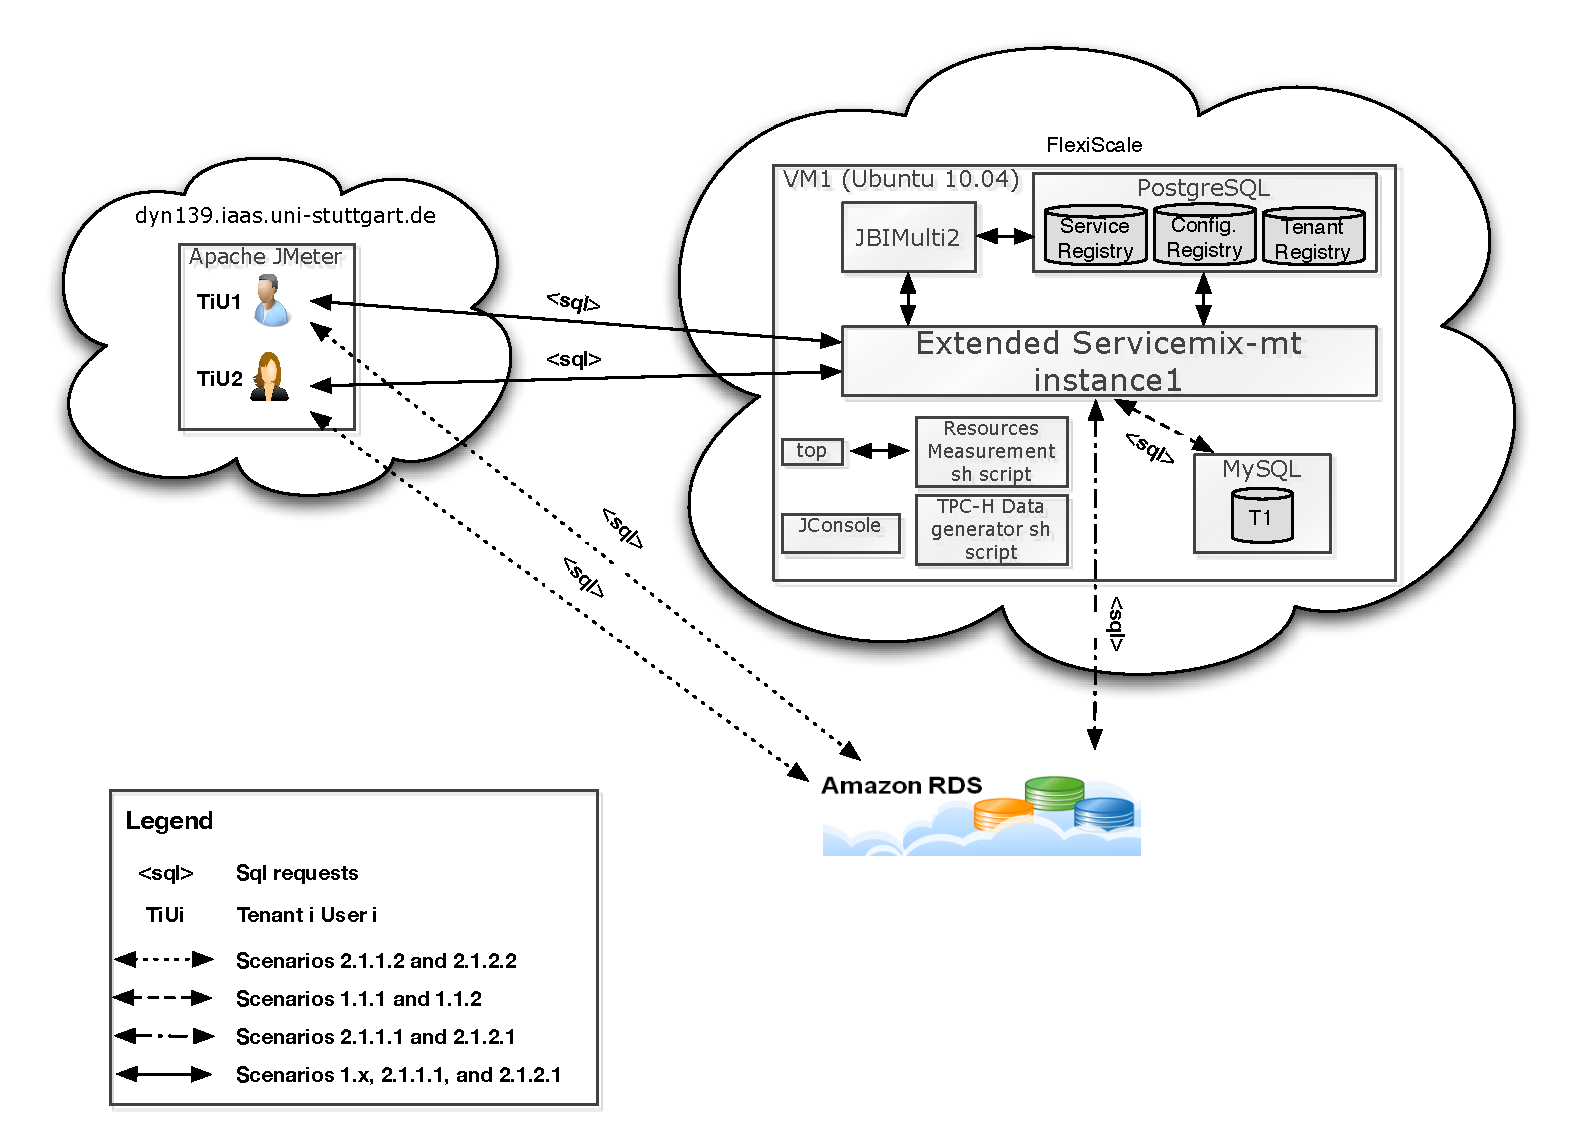
\includegraphics[clip, scale=0.6]{./gfx/evaluationoverview.pdf}
	\caption[Evaluation Architecture Overview]{Evaluation architecture overview for one tenant, two users, and local and remote \ac{SQL} Cloud data store.}
	\label{fig:evaluationoverview}
\end{figure}

The third subsystem is hosted in a VM image in the FlexiScale Cloud infrastructure \cite{flexiscale}. In an Ubuntu 10.04 64 bits operative system with a Java 6 VM we install the following components (see Figure \ref{fig:evaluationoverview}): 
\begin{itemize}
	\item JOnAS 5.2.2.
	\item PostgreSQL 9.1.1.
	\item Extended version of JBIMulti2
	\item A MySQL 5.1 database system which hosts the tenant 1 database.
	\item Extended version of ServiceMix-mt: we modify its minimum and maximum heap consumption allowance, and set it to minimum 256 MB, and maximum 1 GB.
	\item TPC-H data and query generator.
	\item Resource measurements component
\end{itemize}

The resource measurements component measures the CPU utilization of the ServiceMix-mt Java process. Its memory consumption is measured using the JConsole program provided by the JVM (Java Virtual Machine). In this evaluation we are interested in measuring the heap consumption, rather than the memory which is consumed by the JVM. The TPC-H is not used for measurement purposes, but only for data and query generation purposes.  

The evaluation scenarios are defined in Table \ref{tab:evaluation}. We define 8 different scenarios, which follow the following criteria:
\begin{itemize}
	\item Direct connection to the backend database system vs. connection through ServiceMix-mt.
	\item Number of Users, number of concurrent requests per user, and number of requests per user. 
	\item Data stored in a local MySQL database (in the same instance as ServiceMix-mt) vs. data stored in an Amazon RDS MySQL database instance.
\end{itemize}

\lstinputlisting[label={lst:querytpc},caption={[Evaluation Query]Query included in the MySQL requests of the load generator.},style=xml]{./gfx/tpcquery.txt}

The evaluation includes the measurements for the following performance units: throughput (requests per second), data transfer speed (KB/sec), CPU utilization (\%), and Memory utilization (MB). Furthermore, the scenarios are run utilizing the same data retrieval query, which is detailed in Listing \ref{lst:querytpc}.

\begin{table}[htbp]
\centering
\begin{tabular}{llllll}

	\toprule
	Id 		& User num.	& Threads / user		& Req. / thread 		& Backend database	& Through ESB\\
	 \midrule
	 
	 1.1.1.1 						& 2 		& 20						& 100			& Local MySQL			& Yes\\
	 1.1.1.2 						& 2 		& 20						& 100			& Local MySQL			& No\\
	 1.1.2.1 						& 2 		& 50						& 200			& Local MySQL			& Yes\\
	 1.1.2.2 						& 2 		& 50						& 200			& Local MySQL			& No\\
	 2.1.1.1						& 2		& 20						& 100			& MySQL Amazon RDS	& Yes\\
	 2.1.1.2						& 2 		& 20						& 100			& MySQL Amazon RDS	& No	\\
	 2.1.2.1						& 2 		& 50						& 200			& MySQL Amazon RDS	& Yes\\
	 2.1.2.2						& 2 		& 50						& 200			& MySQL Amazon RDS	& No\\
	 
	 
	\bottomrule
\end{tabular}
\caption[CDASMix Evaluation Performance Scenarios]{Specification of the different scenarios to be evaluated. \textbf{Note: } Evaluated the performance for connection through CDASMix and direct to Amazon RDS \cite{amazonrds}.}
	\label{tab:evaluation}
\end{table}

\FloatBarrier

\subsection{Evaluation Analysis}

In this subsection we discuss and present the evaluation results obtained from the execution of the scenarios described in Table \ref{tab:evaluation}. Before getting into the discussion, we point out a problem in the evaluation, which leads us to discard the scenario 2.1.2.2 (see Table \ref{tab:evaluation}). The throughput obtained in the scenario 2.1.1.2 (see Table \ref{tab:evaluation}) is in average 3,3 requests per minute, and lasts approximately 10 hours. This fact makes us delete the last scenario execution, due to the low performance obtained, which we assume that it is related with the Quality of Service assigned to the student grants credits profile in Amazon RDS. 

As it can be seen in Figure \ref{fig:throughput}, utilizing ServiceMix-mt as the database layer component for communicating with a MySQL database system locally deployed lowers the throughput in a 32,74 \% for 2 users, 20 concurrent threads per user, and 100 requests per thread. However, when the thread and request number are increased, the throughput exponentially decreases, as we reach the limit of concurrent connections supported in the MySQL CDASMix Proxy. When we compare it with a direct connection to a locally deployed MySQL database system, we can see that the concurrent requests are better handled by the MySQL server. In case of avoiding cashing support in ServiceMix-mt, the throughput would considerably decrease when increasing the load. When the distance between the different layers of the application increases, e.g. accessing a database layer deployed in a Cloud infrastructure A, and the database system is located in a Cloud infrastructure B, the number of requests per second decreases (see scenario 2.1.1.1 in Figure \ref{fig:throughput}). However, the difference we obtain from hosting the database layer on premise, but accessing a database system off-premise is 98,64 \% worse, if we compare if with the access through ServiceMix-mt. We must denote that in these scenarios there is a high temporal proximity of equal requests. Therefore, the cashing mechanism in the system increases considerably the throughput when accessing data hosted off-premise through ServiceMix-mt.
 
\begin{figure}[htb]
	\centering
		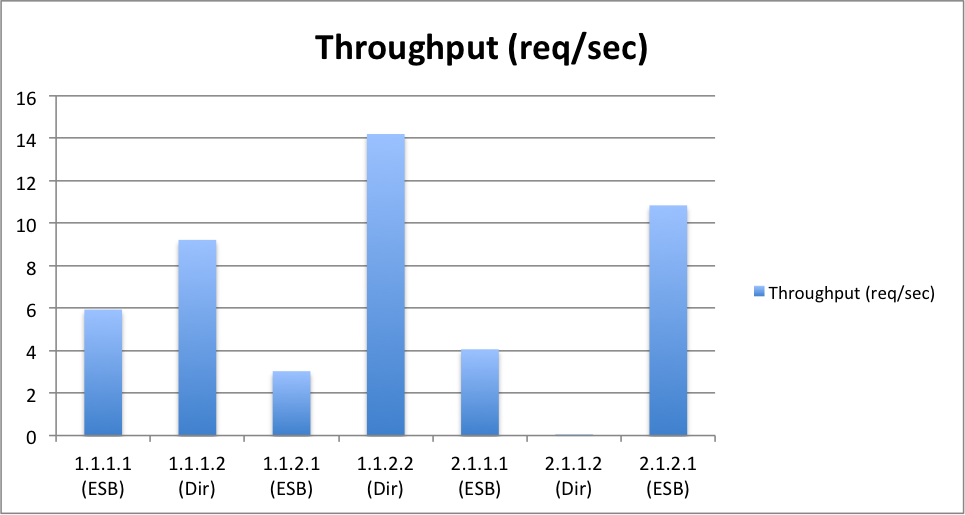
\includegraphics[clip, scale=0.8]{./gfx/throughput.png}
	\caption[Evaluation Analysis - Throughput]{Throughput (requests per second) for the different scenarios described in Table \ref{tab:evaluation}.}
	\label{fig:throughput}
\end{figure}

\FloatBarrier

The amount of KB per second transmitted in the different scenarios correlates with the tendency which can be seen in throughput (see Figures \ref{fig:throughput} and \ref{fig:kbs}).

\begin{figure}[htb]
	\centering
		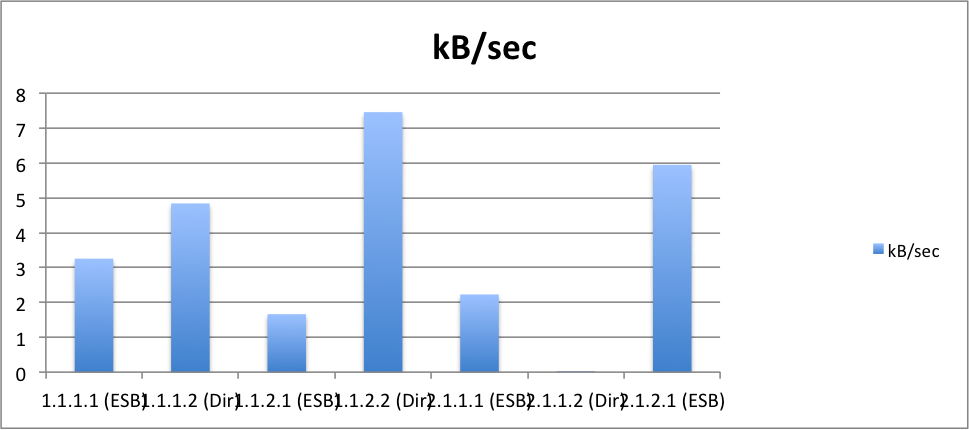
\includegraphics[clip, scale=0.8]{./gfx/kbs.png}
	\caption[Evaluation Analysis - Transmission Speed]{Transmission speed (KB per second) for the different scenarios described in Table \ref{tab:evaluation}.}
	\label{fig:kbs}
\end{figure}

\FloatBarrier

Memory utilization maintains stable along the different scenarios. We observe that in non of the scenarios the maximum heap size (1 GB) is reached in maximum or average values (see Figure \ref{fig:memory}). We obtain a lower memory utilization for the scenarios where data retrieval from a backend Cloud data store is involved. This difference relies on the network latency of having the data hosted in a database system which is not in the same network (in our evaluation, the database instance hosted in Amazon RDS), and the low network latency of having the database system in the same machine as the database layer. A greater number of threads handling the routing requests are blocked due to a higher response time when accessing a remote database system. 

\begin{figure}[htb]
	\centering
		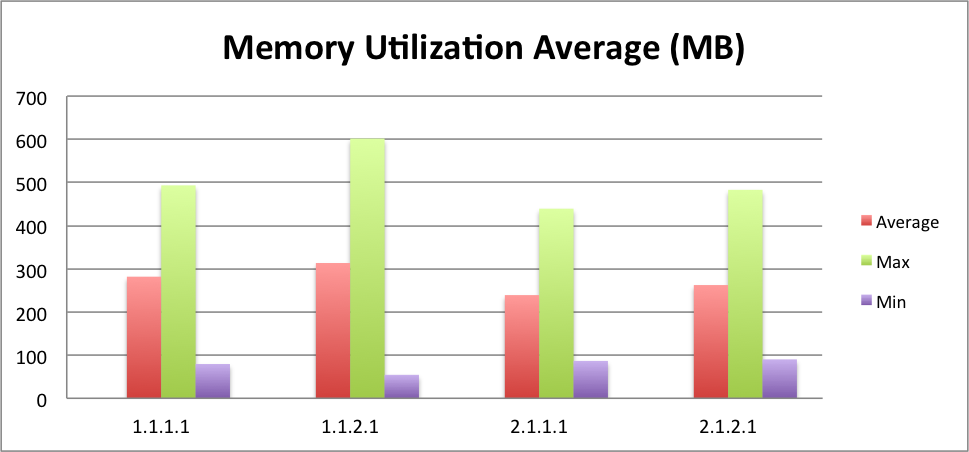
\includegraphics[clip, scale=0.8]{./gfx/memory.png}
	\caption[Evaluation Analysis - Memory Utilization]{Memory utilization (MB) for the different scenarios described in Table \ref{tab:evaluation} where ServiceMix-mt is involved.}
	\label{fig:memory}
\end{figure}

The same difference seen in the memory utilization can be observed in the CPU consumption (see Figure \ref{fig:cpuutilization}). When the requests are executed on a local database system, the response time per request is highly lower than a response time from a remote database. Therefore, the CPU utilization averages and maximum values are closer to each other. However, when accessing the MySQL database instance in Amazon RDS, the maximum values correlate with the scenarios 1.1.1.1 and 1.1.2.1, but in average the CPU utilization is lower due to a higher number of blocked threads.

\begin{figure}[htb]
	\centering
		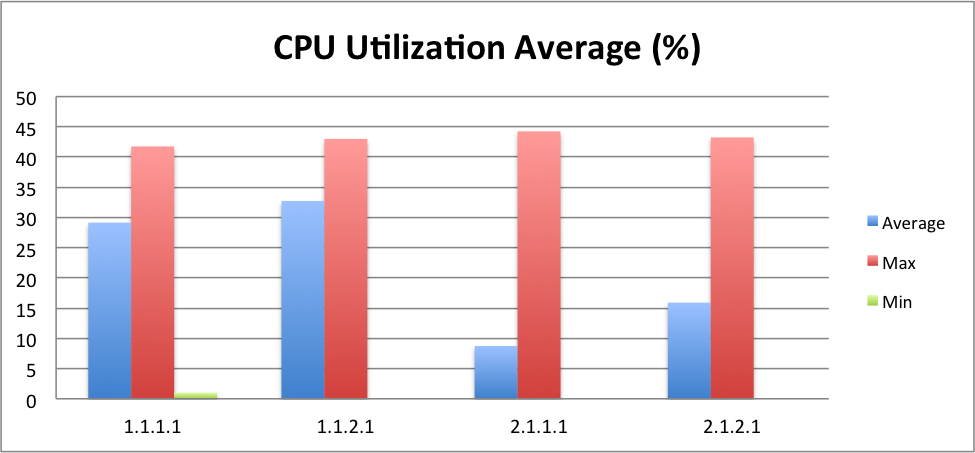
\includegraphics[clip, scale=0.8]{./gfx/cpuutilization.png}
	\caption[Evaluation Analysis - CPU Utilization]{CPU utilization (\%) for the different scenarios described in Table \ref{tab:evaluation} where ServiceMix-mt is involved.}
	\label{fig:cpuutilization}
\end{figure}

\FloatBarrier